\documentclass[a4paper, 12pt]{article}

% --- CÁC GÓI THƯ VIỆN CẦN THIẾT ---
\usepackage[T5]{fontenc} 
\usepackage[utf8]{inputenc}
\usepackage{graphicx} 
\usepackage{geometry} 
\geometry{a4paper, left=2.5cm, right=2cm, top=2.5cm, bottom=2.5cm}
\usepackage{hyperref} 
\usepackage{listings} 
\usepackage{color}
\usepackage{float}

\begin{document}

\title{\textbf{Kiểm thử và So sánh hiệu năng các chuẩn Wi-Fi trên thiết bị thực tế (D-LINK DWR-700}}
\author{Thực hiện: Tom Nguyen}
\date{Tháng 4 năm 2026}

\maketitle

\section{Tổng quan quá trình kiểm thử}
Sau khi tìm hiểu nguyên lý hoạt động trên phần mềm mô phỏng, chúng ta tiến hành kiểm chứng lại các lý thuyết này trên thiết bị phát sóng vô tuyến thực tế. Do giới hạn về mặt phần cứng của thiết bị, bài kiểm thử này sẽ tập trung phân tích và so sánh hai chuẩn mạng hoạt động trên cùng băng tần 2.4GHz là chuẩn 802.11b và chuẩn 802.11g.

Mô hình thiết bị bao gồm:
\begin{itemize}
    \item \textbf{Bộ phát sóng trung tâm:} Thiết bị định tuyến (DWR-700) được truy cập vào trang quản trị (địa chỉ 192.168.0.1) để chủ động ép mạng phát sóng độc lập theo từng chuẩn.
    \item \textbf{Thiết bị đầu cuối:} Điện thoại thông minh chạy hệ điều hành Android, cài đặt sẵn các ứng dụng phân tích mạng lưới.
    \item \textbf{Máy tính cá nhân:} Kết nối bằng dây cáp vào bộ phát sóng, đóng vai trò làm máy chủ lưu trữ cục bộ.
\end{itemize}

\section{Các bài thí nghiệm và Phân tích kết quả}

\subsection{Đo lường cường độ tín hiệu và suy hao do khoảng cách}
Ứng dụng kiểm tra hệ thống trên điện thoại được sử dụng để đọc các thông số trực tiếp từ card mạng không dây. Chúng ta tiến hành đo đạc ở hai vị trí: ngay sát bộ phát sóng ở khoảng cách 0.2 mét và cách xa 10 mét.

\begin{figure}[H]
    \centering
    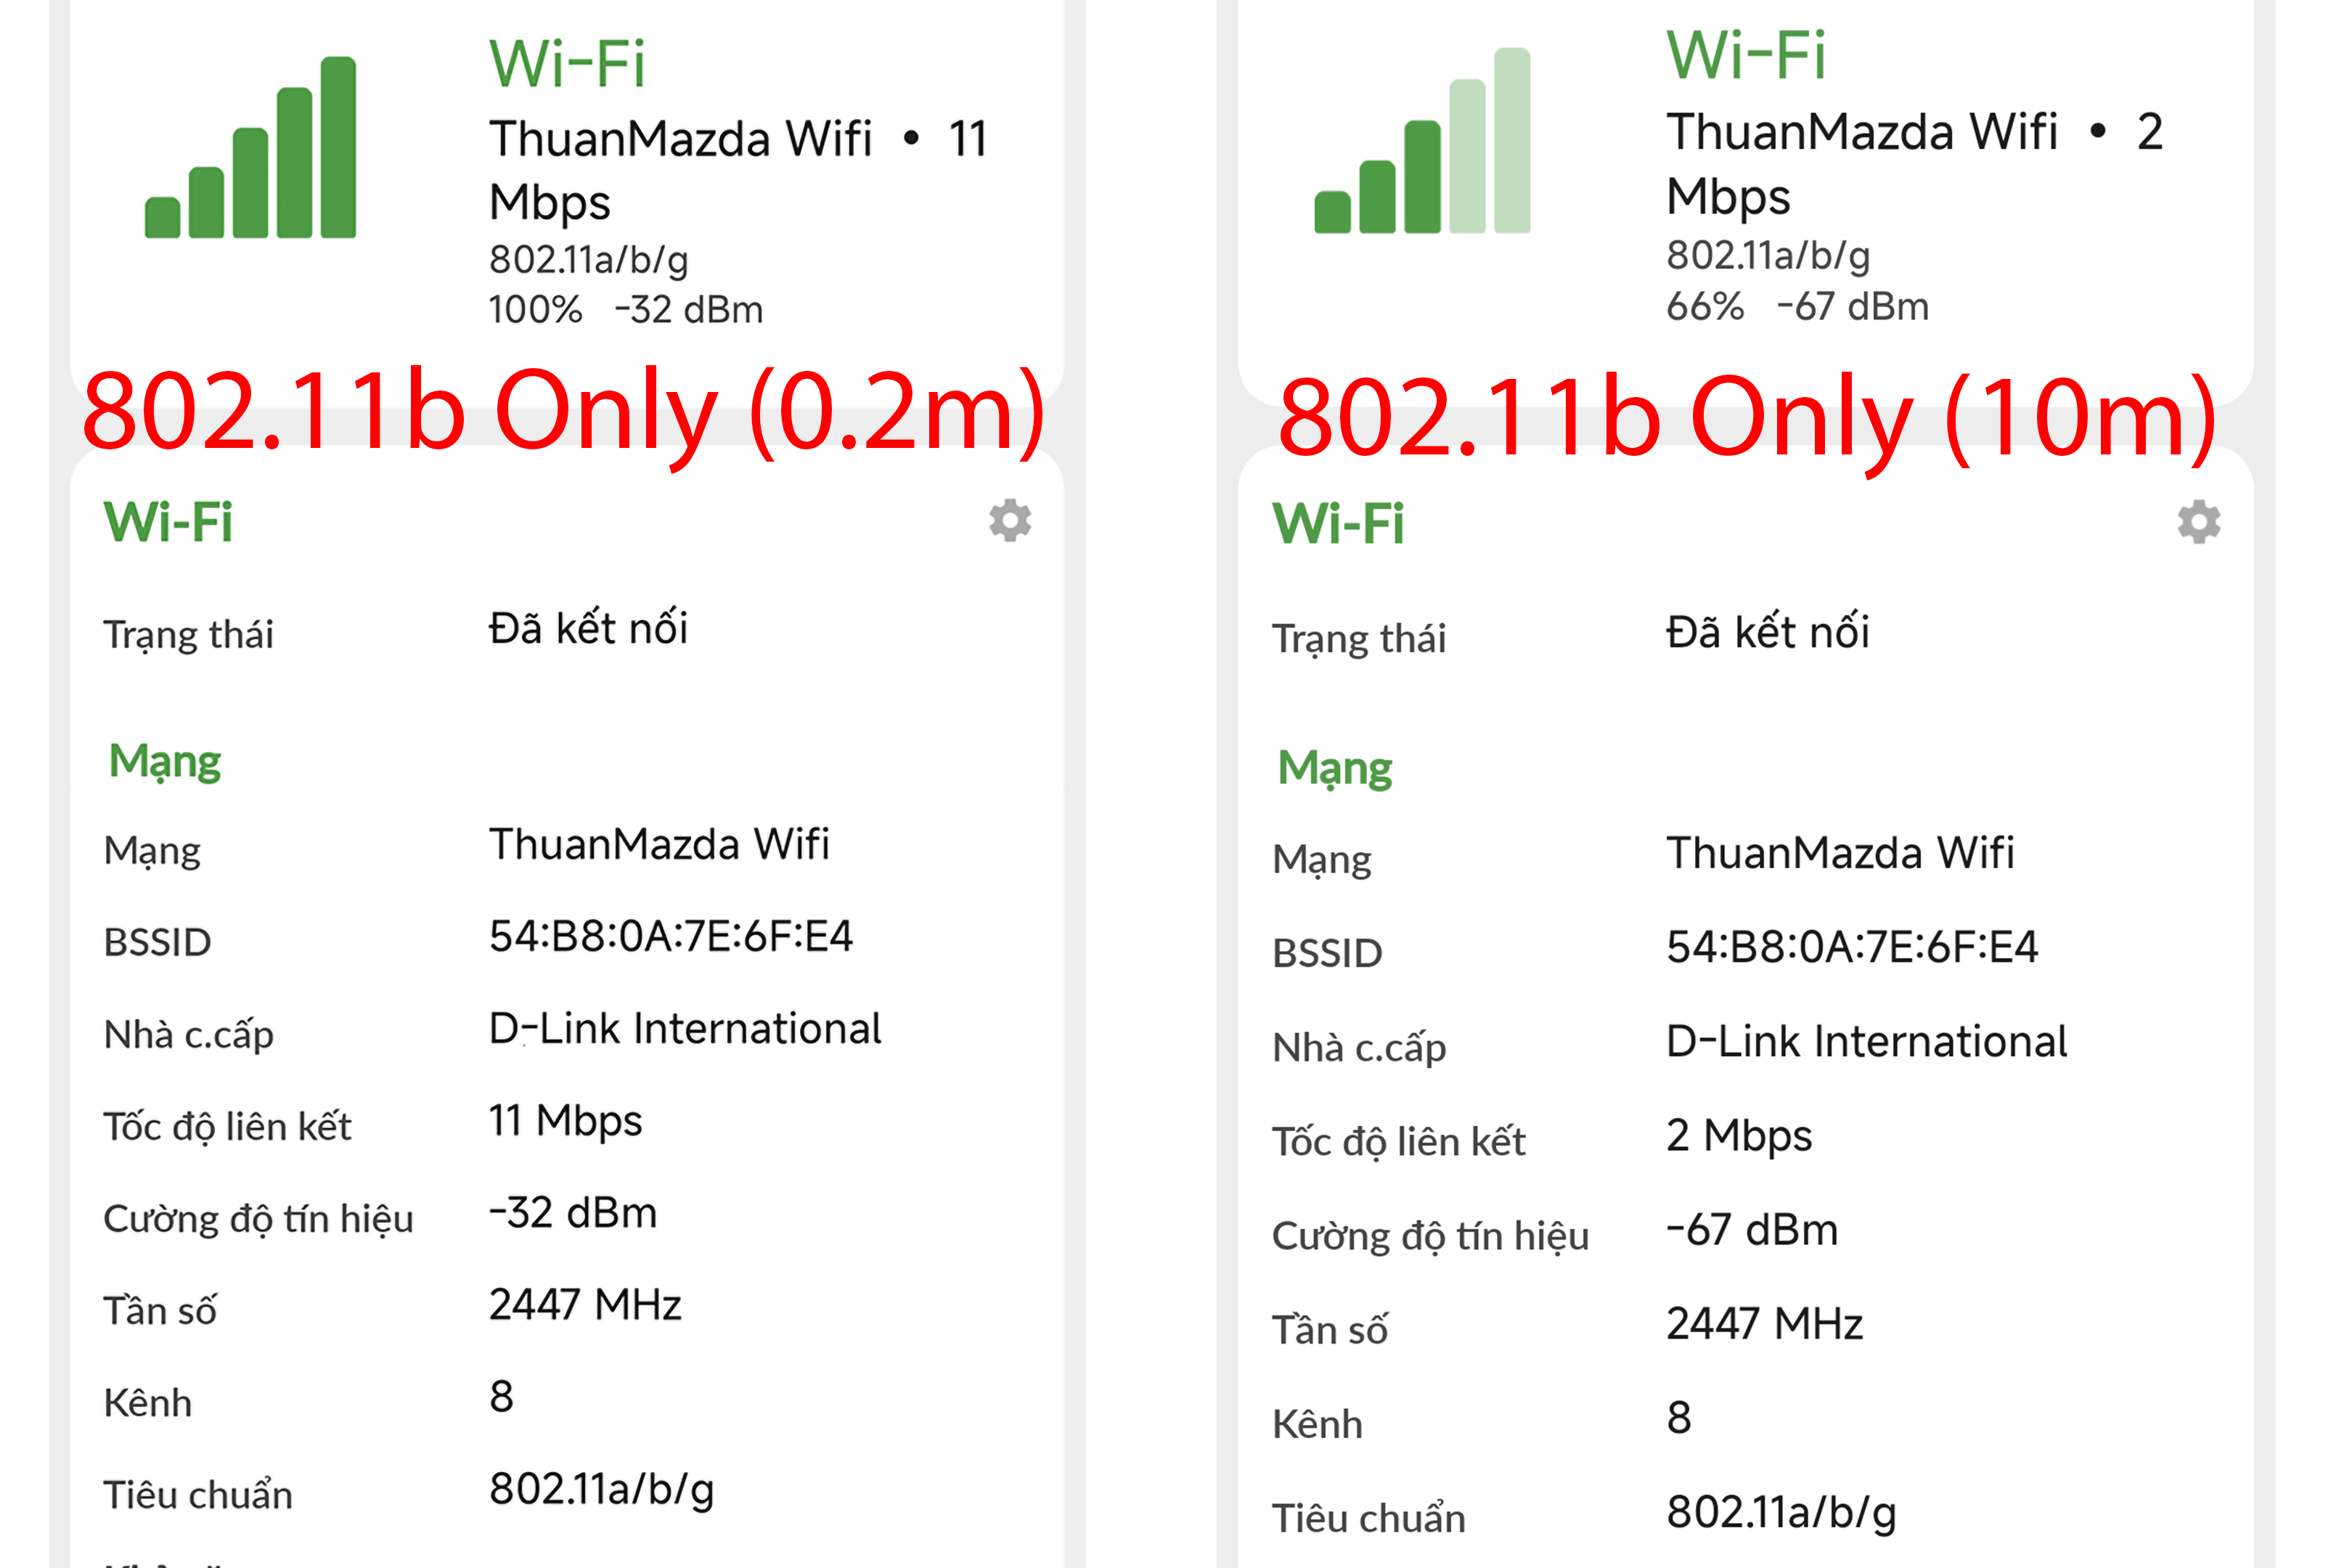
\includegraphics[width=0.97\textwidth]{Fig1.jpg}
    \caption{So sánh cường độ tín hiệu mạng chuẩn 802.11b qua ứng dụng phân tích phần cứng}
\end{figure}

\begin{figure}[H]
    \centering
    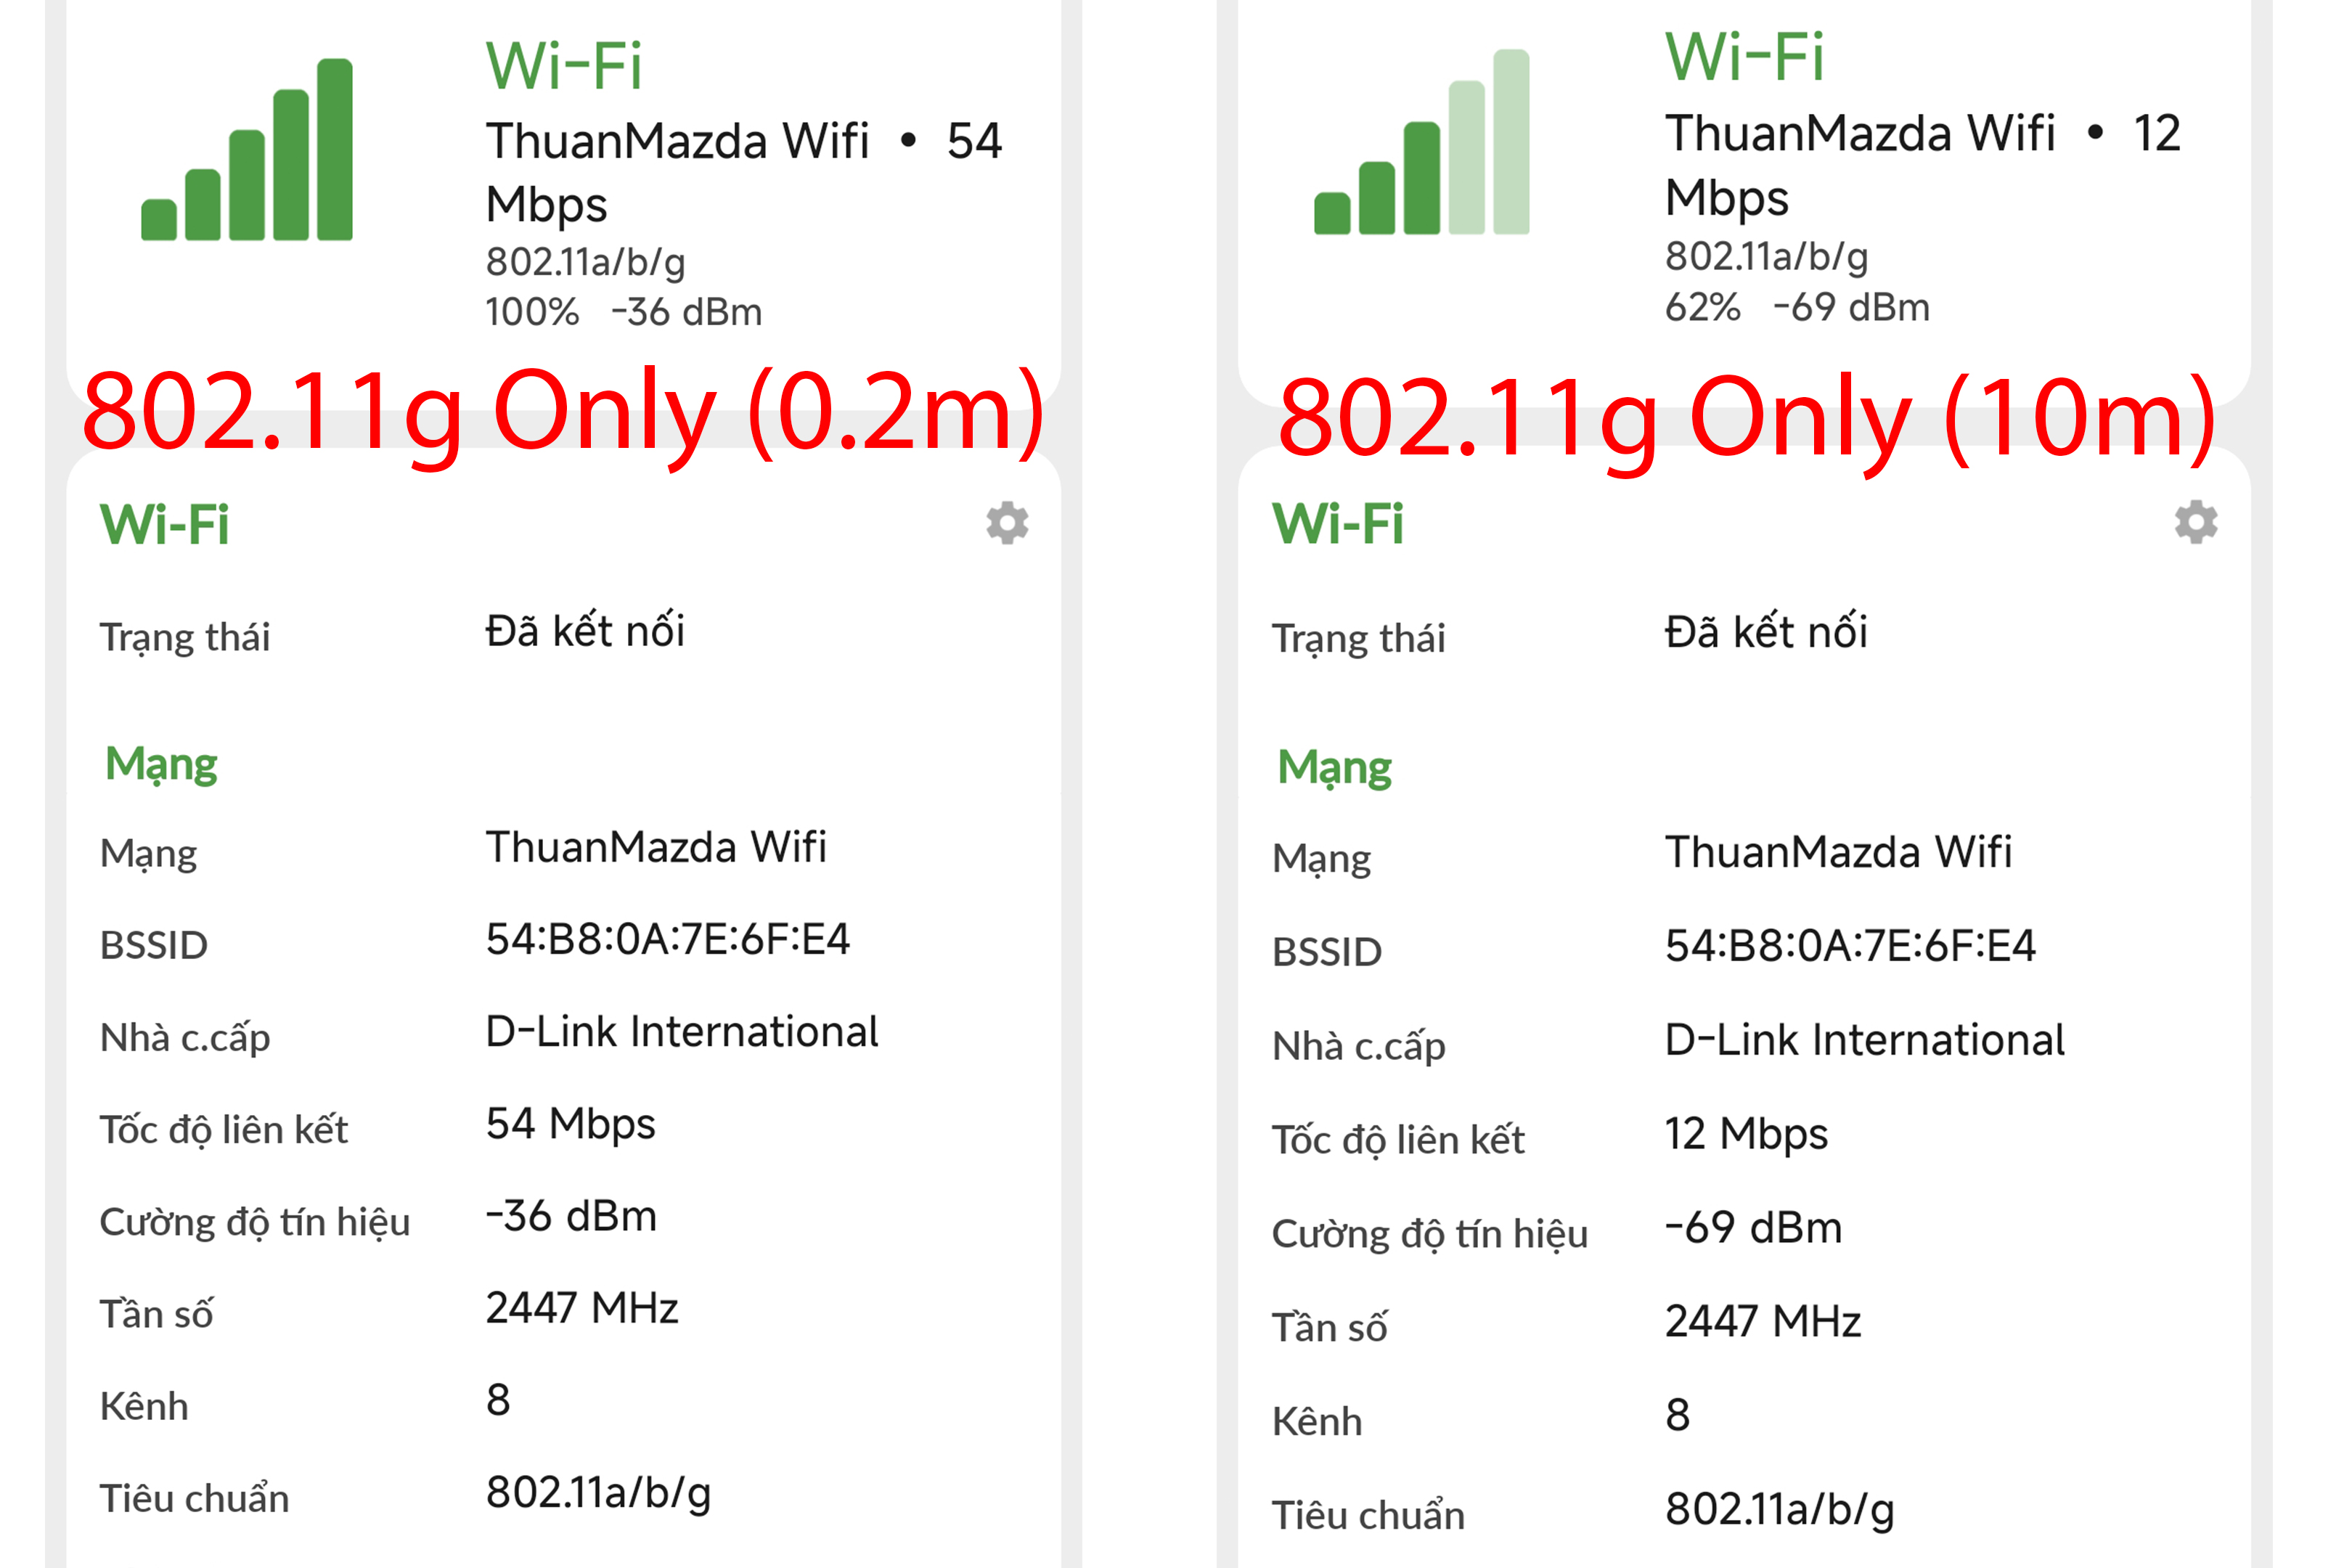
\includegraphics[width=0.97\textwidth]{Fig2.jpg}
    \caption{So sánh cường độ tín hiệu mạng chuẩn 802.11g qua ứng dụng phân tích phần cứng}
\end{figure}

\textbf{Nhận xét kết quả đo lường:}
Dựa vào các chỉ số ghi nhận được từ phần mềm, chúng ta có thể rút ra hai kết luận quan trọng về đặc tính của sóng vô tuyến:

\begin{itemize}
    \item \textbf{Về cường độ tín hiệu:} Vì cả hai chuẩn đều hoạt động trên cùng một kênh truyền tần số 2447 MHz thuộc băng tần 2.4 GHz, nên sự suy hao năng lượng khi đi qua môi trường vật lý là hoàn toàn tương đồng. Ở khoảng cách cực gần 0.2 mét, tín hiệu thu được rất khỏe, đạt mức -32 dBm đối với chuẩn b và -36 dBm đối với chuẩn g. Khi chúng ta di chuyển ra xa 10 mét, tín hiệu của cả hai đều suy giảm mạnh và rơi xuống mức xấp xỉ nhau là -67 dBm và -69 dBm.
    
    \item \textbf{Về tốc độ liên kết:} Đây là minh chứng rõ ràng nhất cho sự khác biệt về công nghệ điều chế tín hiệu. Ở khoảng cách lý tưởng, chuẩn 802.11g phát huy tối đa sức mạnh với tốc độ liên kết đạt 54 Mbps, cao gấp gần năm lần so với mức trần 11 Mbps của chuẩn 802.11b. Khi ra xa 10 mét và cường độ sóng suy yếu, cả hai chuẩn mạng đều buộc phải tự động hạ bậc điều chế để duy trì tính toàn vẹn của dữ liệu. Chuẩn 802.11b sụt giảm nghiêm trọng xuống chỉ còn 2 Mbps mỗi giây. Trong khi đó, chuẩn 802.11g giảm xuống mức 12 Mbps mỗi giây. Điều này cho thấy ngay cả trong điều kiện sóng yếu, nền tảng công nghệ mới hơn vẫn đảm bảo một mức băng thông kết nối vượt trội so với chuẩn cũ.
\end{itemize}

\subsection{Kiểm tra độ trễ mạng cục bộ}
Để kiểm tra tốc độ phản hồi của môi trường vô tuyến, chúng ta sử dụng công cụ mạng trên điện thoại để gửi các gói tin có kích thước rất nhỏ (64 byte) liên tục đến địa chỉ của bộ phát sóng trung tâm. Bài kiểm tra này được thực hiện ở khoảng cách cực gần, ngay sát bộ phát vô tuyến.

\begin{figure}[H]
    \centering
    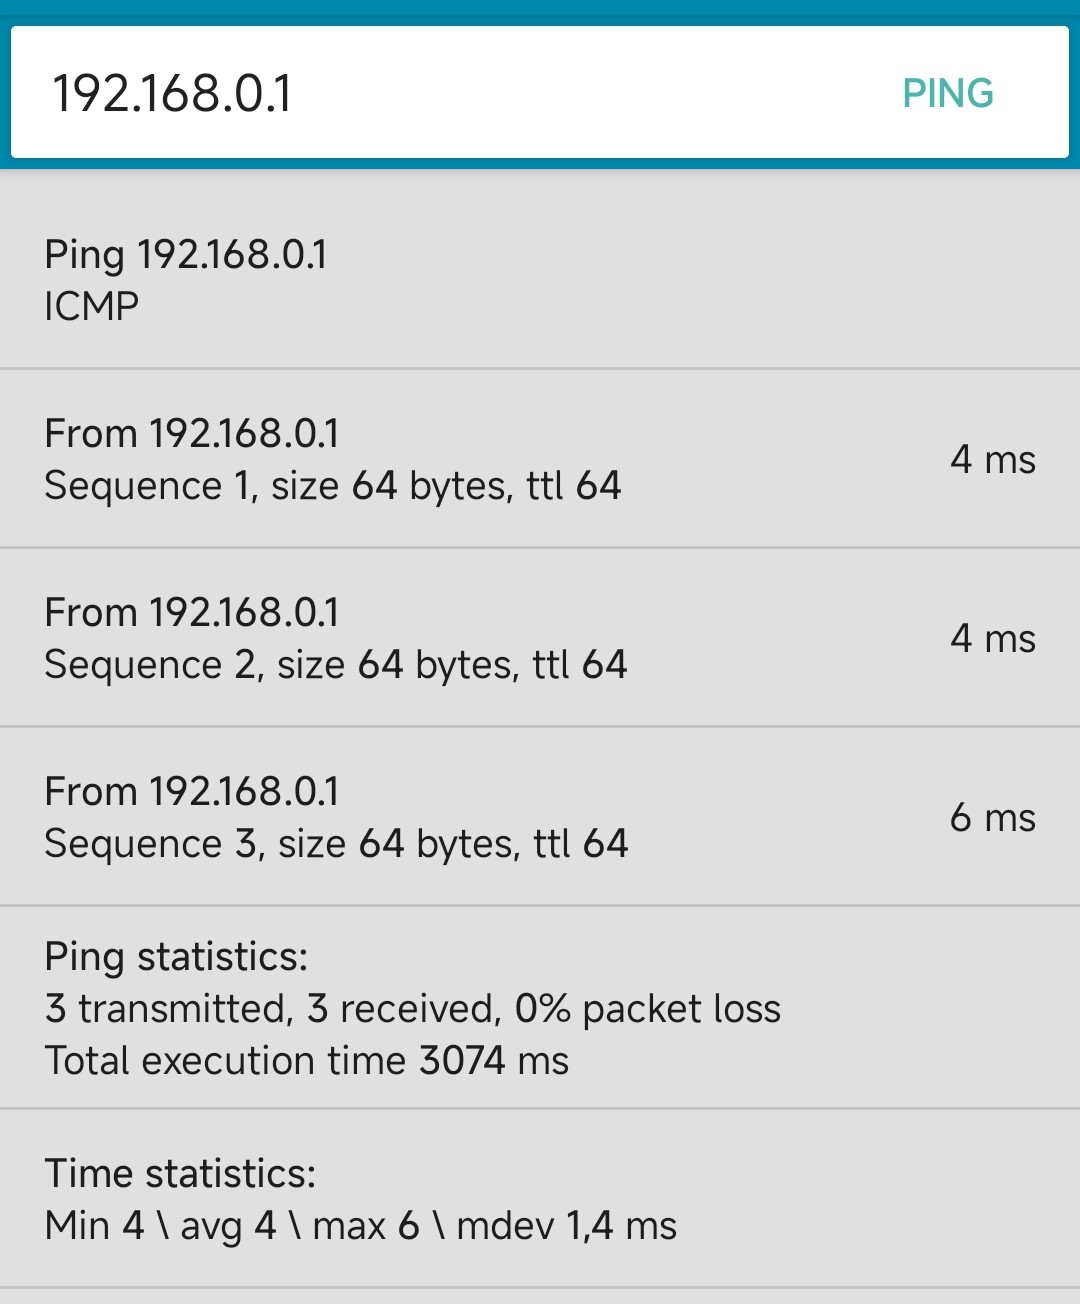
\includegraphics[width=0.52\textwidth]{Fig3.jpg}
    \caption{Kết quả đo độ trễ mạng nội bộ chuẩn 802.11b đến máy chủ trung tâm}
\end{figure}

\begin{figure}[H]
    \centering
    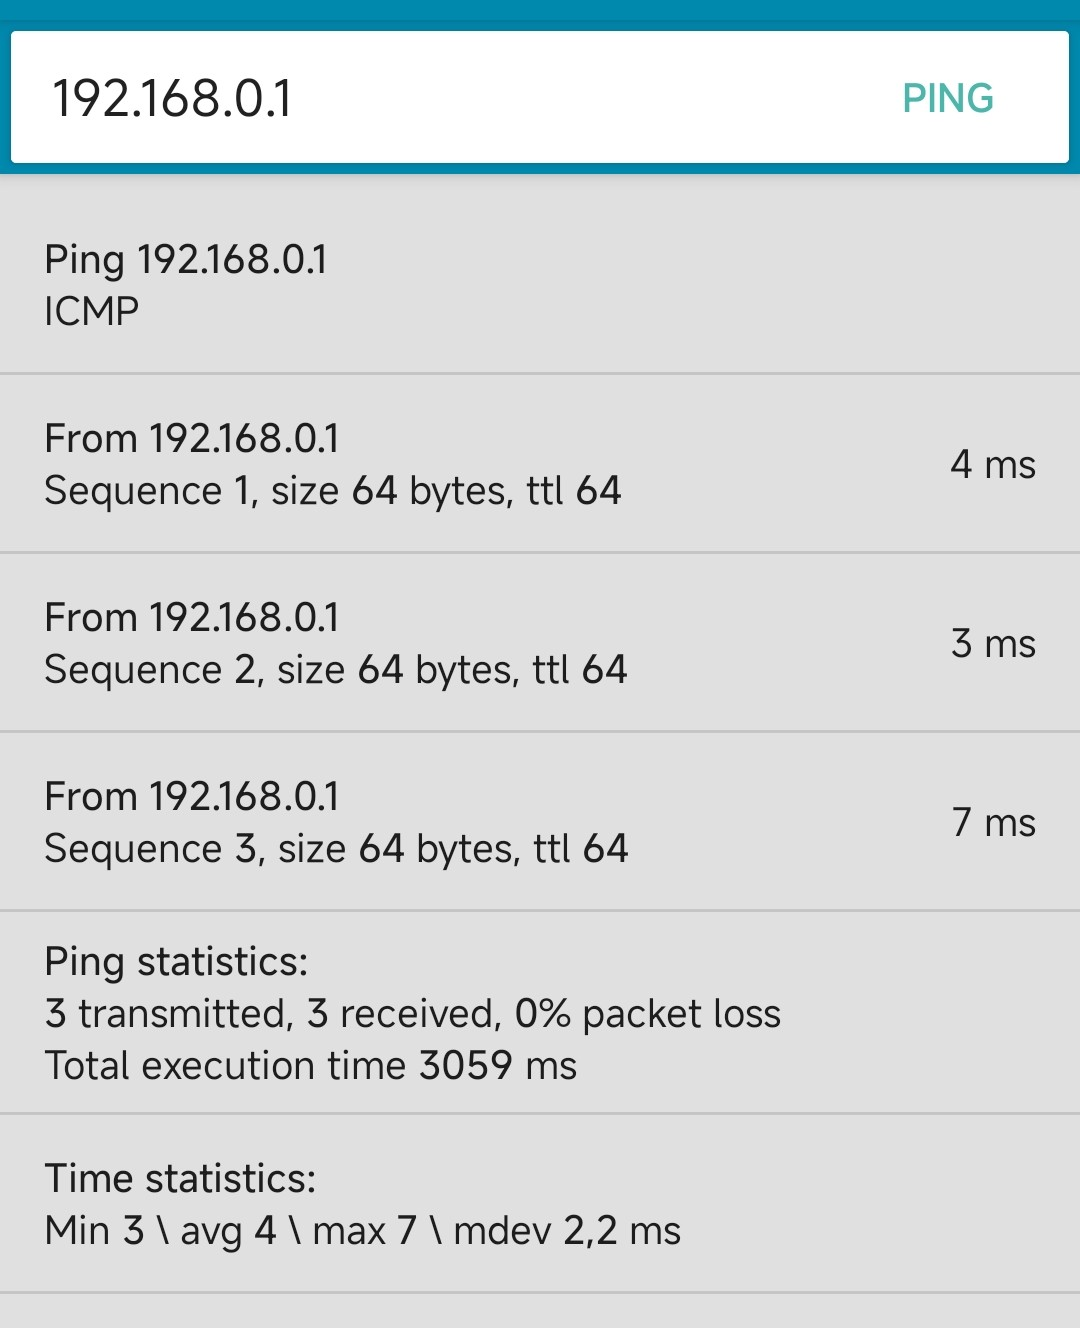
\includegraphics[width=0.52\textwidth]{Fig4.jpg}
    \caption{Kết quả đo độ trễ mạng nội bộ chuẩn 802.11g đến máy chủ trung tâm}
\end{figure}

Dựa vào thông số đo đạc trên màn hình, kết quả được phân bổ như sau:
\begin{itemize}
    \item \textbf{Chuẩn 802.11b:} Độ trễ trung bình là 4 mili giây. Mức độ dao động tín hiệu rất thấp và ổn định, chỉ ở mức 1,4 mili giây.
    \item \textbf{Chuẩn 802.11g:} Độ trễ trung bình cũng đạt 4 mili giây. Tuy nhiên, mức độ dao động tín hiệu lại cao hơn, đạt 2,2 mili giây và có thời điểm độ trễ vọt lên mức 7 mili giây.
\end{itemize}

\textbf{Nhận xét kết quả:}
Thoạt nhìn, kết quả này dường như đi ngược lại với logic thông thường, bởi vì một chuẩn mạng cũ hơn lại cho thấy sự ổn định hơn so với chuẩn thế hệ mới. Tuy nhiên, hiện tượng này hoàn toàn có thể lý giải được dựa trên bản chất vật lý của sóng và cách xử lý của phần cứng:
\begin{itemize}
    \item \textbf{Kích thước dữ liệu quá nhỏ:} Gói tin được gửi đi trong bài thử nghiệm này chỉ có dung lượng 64 byte. Với khối lượng dữ liệu siêu nhẹ, điểm yếu về giới hạn băng thông 11 Megabit mỗi giây của chuẩn cũ hoàn toàn không bị bộc lộ, do thời gian truyền tải thực tế chỉ diễn ra trong vòng một phần ngàn giây cho cả hai chuẩn.
    \item \textbf{Độ phức tạp của kỹ thuật điều chế ở cự ly quá gần:} Chuẩn 802.11b sử dụng kỹ thuật điều chế trải phổ chuỗi trực tiếp, một công nghệ tuy tốc độ chậm nhưng xử lý phần cứng rất đơn giản và ổn định. Ngược lại, chuẩn 802.11g sử dụng kỹ thuật ghép kênh phân chia theo tần số trực giao rất phức tạp để đạt được tốc độ cao. Khi đặt thiết bị quá sát bộ phát sóng, tín hiệu cường độ cực mạnh có thể gây ra hiện tượng bão hòa tín hiệu vi mô. Việc phần cứng phải liên tục tính toán, mã hóa và giải mã các luồng sóng phức tạp của chuẩn thế hệ mới trên những gói tin quá nhỏ vô tình tạo ra sự chênh lệch thời gian xử lý vi mô giữa các lần gửi, dẫn đến chỉ số dao động cao hơn đôi chút.
\end{itemize}

Kết luận lại, với các tác vụ chỉ gửi những gói lệnh nhỏ lẻ (như tin nhắn văn bản hay tín hiệu điều khiển nhà thông minh) ở khoảng cách gần, chuẩn công nghệ cũ vẫn hoạt động cực kỳ bền bỉ. Để thấy rõ sự chênh lệch về năng lực truyền tải và chống nhiễu thực sự giữa hai thế hệ, chúng ta buộc phải tiến hành bài thử nghiệm ép tải một tệp dữ liệu lớn.

\subsection{Thí nghiệm đánh giá băng thông truyền tải thực tế}
Để đánh giá chính xác sức mạnh luân chuyển dữ liệu của thiết bị mạng, chúng ta sử dụng một ứng dụng đo lường chuyên dụng trên điện thoại thông minh là \texttt{Wi-fi SweetSpots}. Ứng dụng này liên tục đẩy các khối dữ liệu trực tiếp đến bộ phát sóng trung tâm và tính toán băng thông luân chuyển nội bộ theo thời gian thực. Phương pháp này giúp chúng ta loại bỏ hoàn toàn yếu tố thắt cổ chai từ gói cước của nhà cung cấp dịch vụ viễn thông. Bài kiểm tra được thực hiện hai lần ở cùng một vị trí: một lần ép bộ phát chạy độc lập ở chuẩn b, và một lần chạy độc lập ở chuẩn g.

\begin{figure}[H]
    \centering
    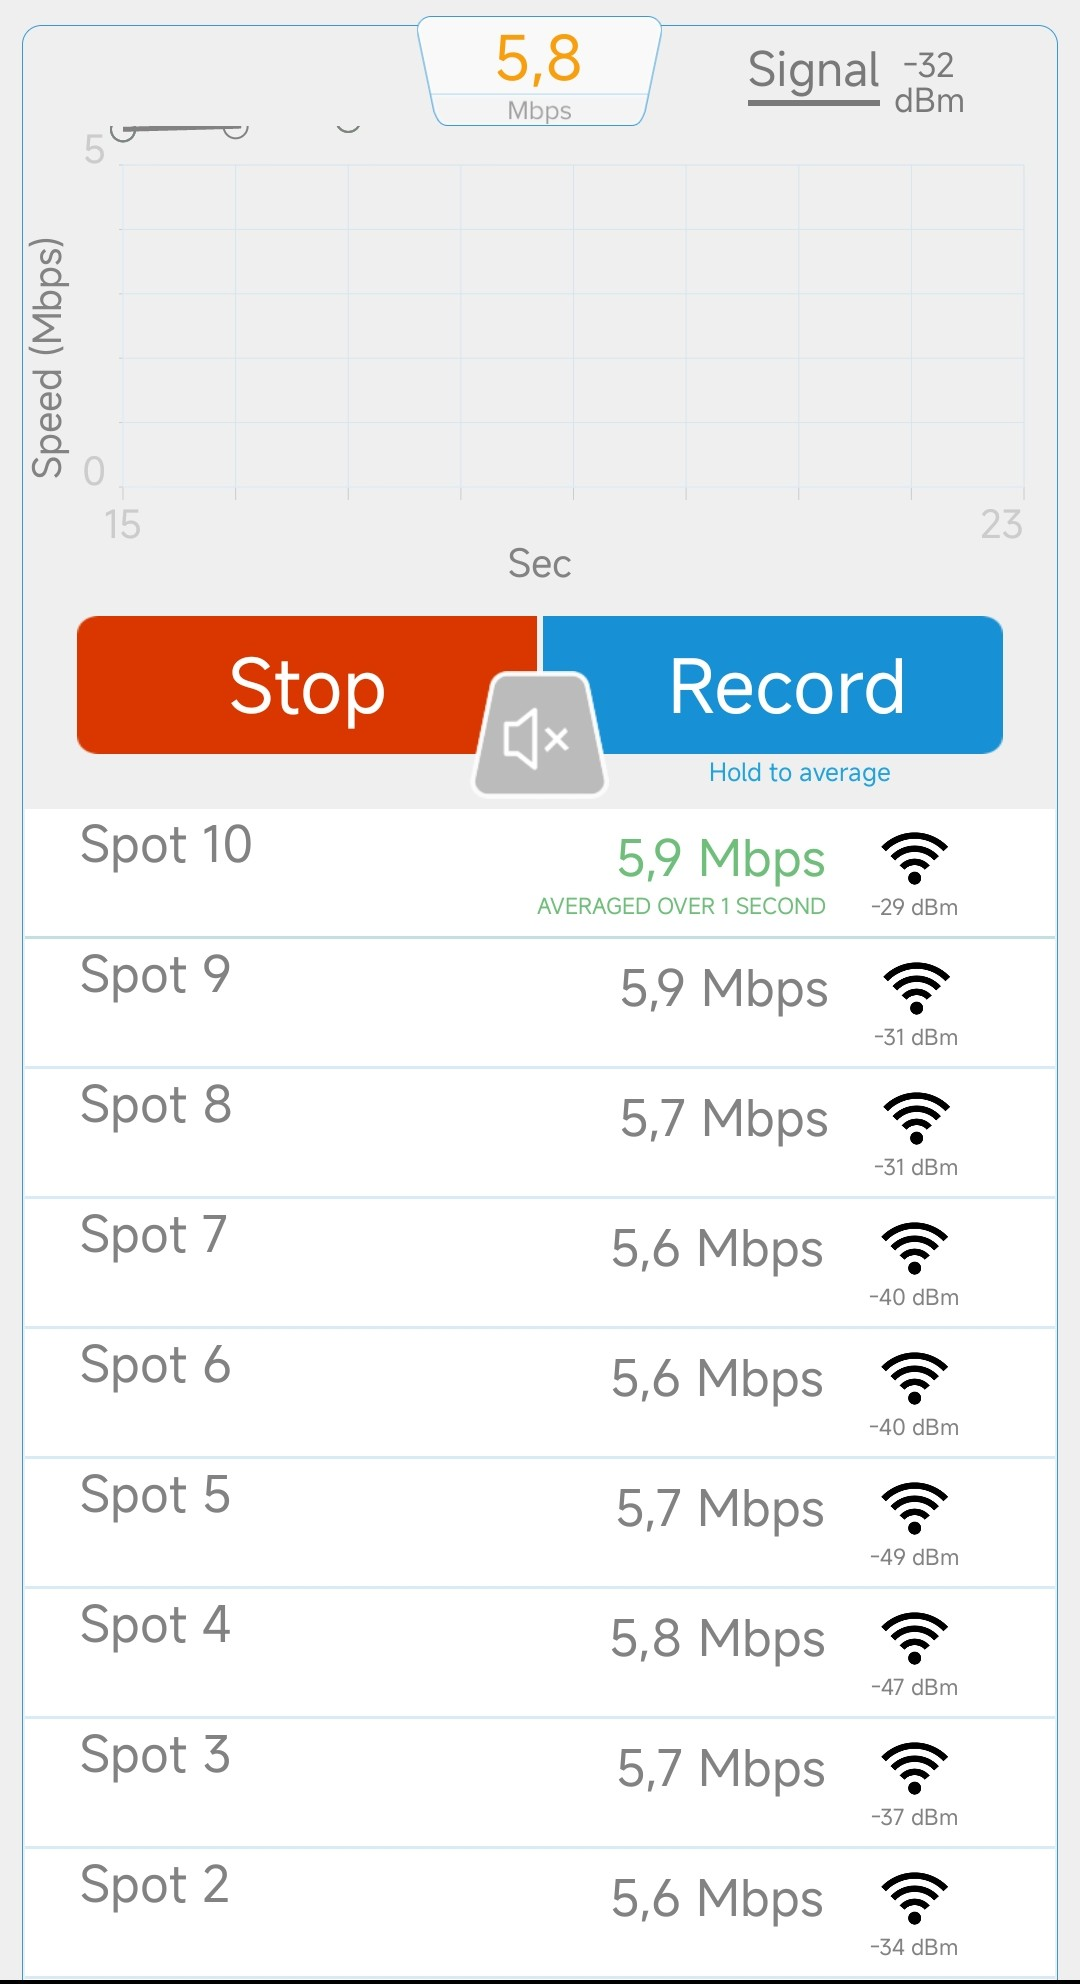
\includegraphics[width=0.49706\textwidth]{Fig5.jpg}
    \caption{Kiểm tra băng thông truyền tải dữ liệu cục bộ của chuẩn 802.11b}
\end{figure}

\begin{figure}[H]
    \centering
    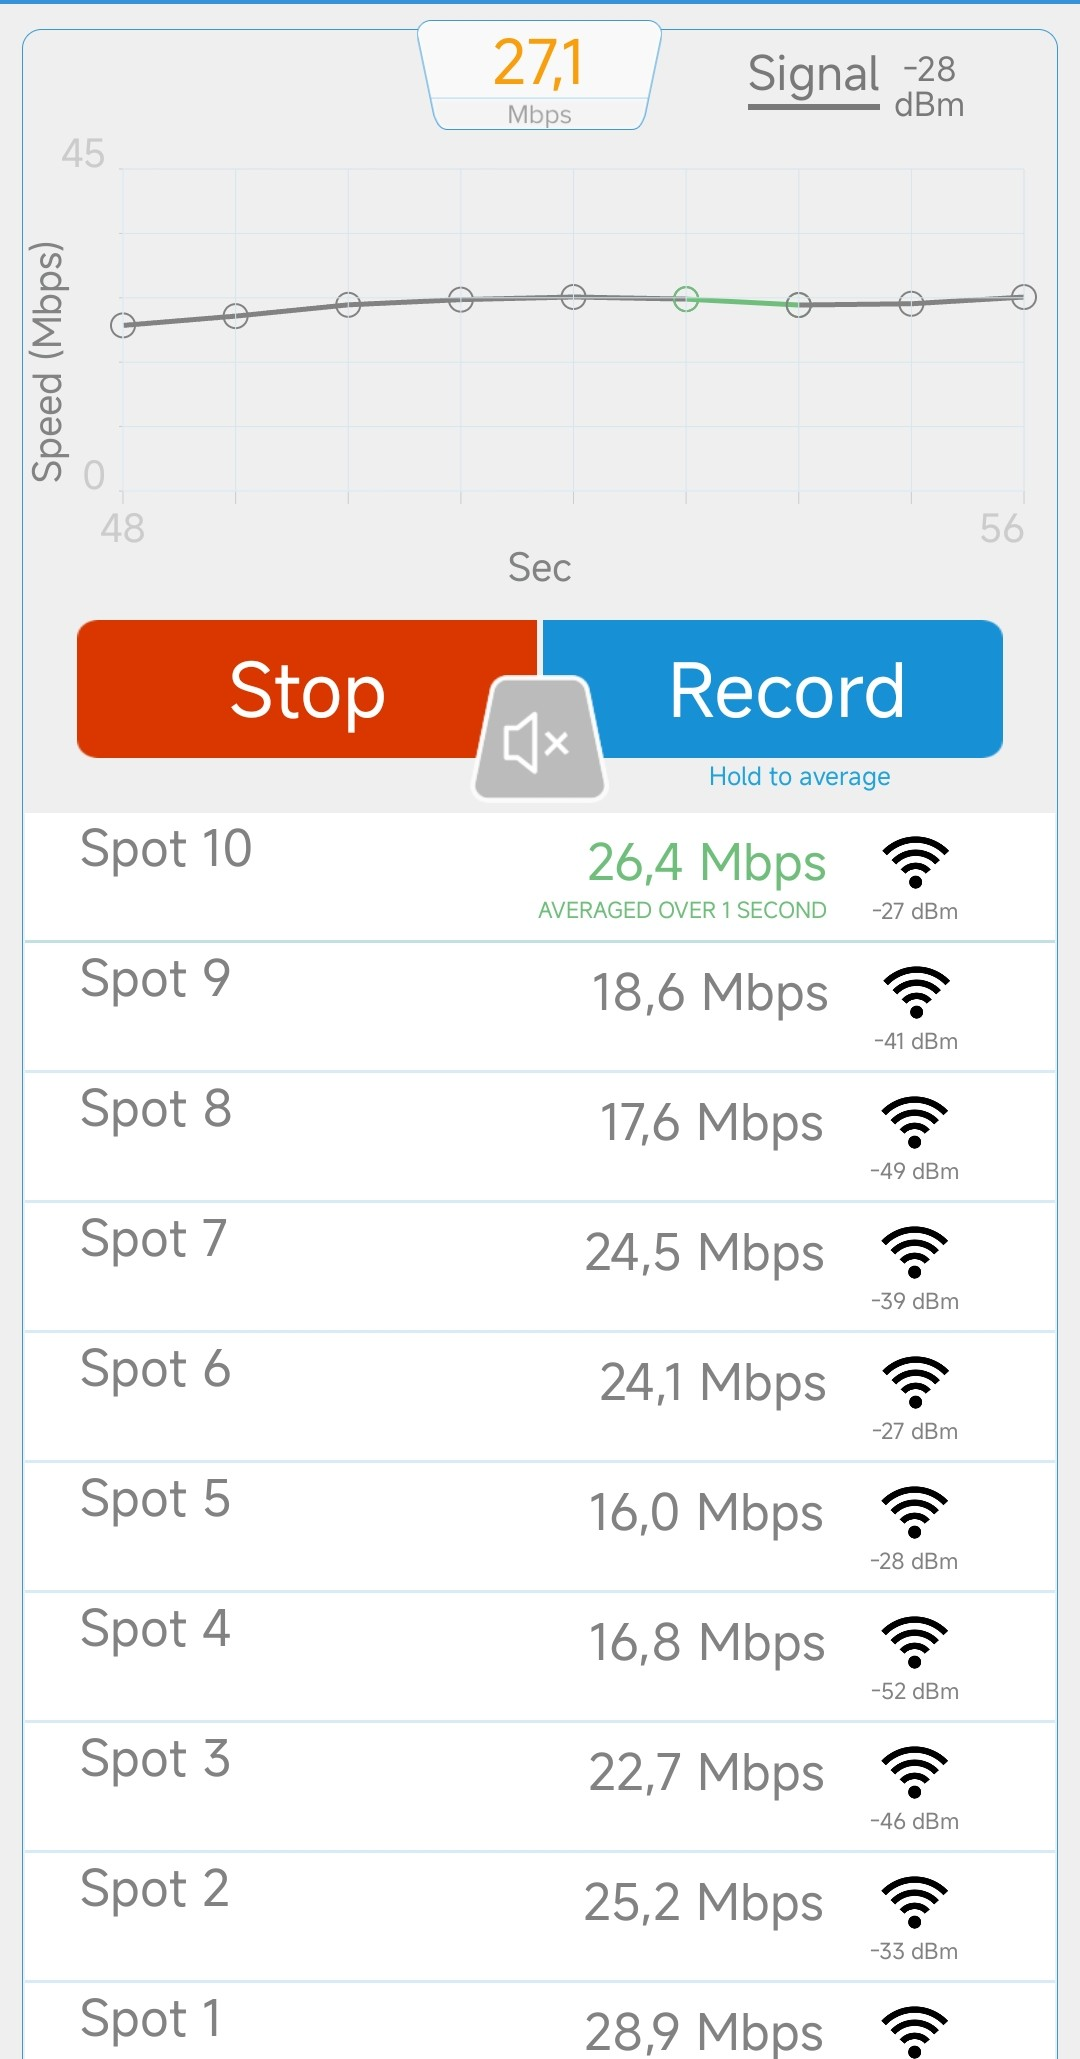
\includegraphics[width=0.49706\textwidth]{Fig6.jpg}
    \caption{Kiểm tra băng thông truyền tải dữ liệu cục bộ của chuẩn 802.11g}
\end{figure}

\textbf{Nhận xét kết quả đo lường:}
Kết quả thu được từ phần mềm đã phản ánh một cách chân thực nhất giới hạn phần cứng của từng thế hệ công nghệ vô tuyến:

\begin{itemize}
    \item \textbf{Ở chuẩn 802.11b:} Mặc dù thiết bị được đặt ở vị trí rất gần với cường độ tín hiệu thu được cực kỳ mạnh là -32 dBm, tốc độ truyền tải thực tế chỉ đi ngang và kịch trần ở mức dao động từ 5.6 đến 5.9 Mbps. Con số này là minh chứng rõ ràng cho sự hạn chế của công nghệ trải phổ chuỗi trực tiếp đời cũ, khiến mạng lưới mất rất nhiều thời gian nếu phải cõng một lượng lớn dữ liệu.
    
    \item \textbf{Khi chuyển sang chuẩn 802.11g:} Ngay khi thay đổi giao thức, tốc độ đo đạc thực tế lập tức tăng vọt lên mức trung bình khoảng 27 Megabit mỗi giây, và có những thời điểm chạm ngưỡng gần 29 Mbps. Tốc độ này nhanh gấp gần năm lần so với chuẩn cũ. Sự vượt trội này có được là nhờ kỹ thuật điều chế phân chia tần số trực giao hiện đại, giúp thiết bị tận dụng triệt để kênh truyền để đẩy một lượng lớn khối dữ liệu đi trong cùng một khoảng thời gian.
\end{itemize}

\section{Kết luận thực nghiệm}

Trong thí nghiệm kiểm tra tốc độ ping, chúng ta sẽ nhận thấy với các gói dữ liệu nhỏ, sự chênh lệch giữa chuẩn đời mới hơn và cũ hơn không đáng kể. Nhưng đến thí nghiệm đo băng thông thực tế với các gói tin lớn (dữ liệu chúng ta sử dụng hàng ngày) thì có thể thấy rõ sự khác biệt hẳn giữa chuẩn G và chuẩn B.

Việc mang các bài kiểm tra từ môi trường mô phỏng ra môi trường thực tế đã giúp chúng ta có cái nhìn toàn diện hơn về sóng vô tuyến. Các thông số lý thuyết chỉ mang tính chất tham khảo, hiệu năng thực tế phụ thuộc rất nhiều vào khoảng cách, công nghệ điều chế chống nhiễu và cách thức chia sẻ kênh truyền giữa các thiết bị đầu cuối. 

\end{document}